\chapter{Segundo núcleo: Placa I/O} \chapterlabel{2do-Nucleo} \label{cap:2do-nucleo}

\hl{FALTAN COMPLETAR ALGUNAS COSAS}

En el presente capítulo se tratarán los aspectos relacionados con el desarrollo del segundo gran núcleo del proyecto. El mismo consiste en el diseño y construcción de la placa encargada de controlar los equipos a ubicados en las zonas de ingreso y egreso del establecimiento. Se presentan los esquemas circuitales correspondientes a la fuente de alimentación y a la parte lógica de la placa. Finalmente, se analizan los diversos periféricos comerciales que se encuentran implementados en el sistema, y que son administrados por ella. 

\section{Componentes principales}
En esta primera sección se realiza un breve análisis acerca de los dos principales elementos que constituyen la placa de control. Los mismos son el microcontrolador y el módulo de comunicación WiFi. 

\subsection{Microcontrolador}
Para el reconocimiento del estado de los periféricos del sistema y el uso de dicha información para controlar la ejecución de diversas acciones se escogió el microcontrolador de 8 bits Atmega328P. El mismo es fabricado por la empresa Atmel. El microcontrolador cuenta con 28 pines, de los cuales 23 son líneas de entrada-salida programables. De ellas, 14 son digitales. De estas últimas, dos pertenecen a un puerto serial USART, utilizado para la transmisión de datos con el módulo de comunicación WiFi. Adicionalmente, se utilizan 11 pines digitales para el sensado del estado de los periféricos y la distribución de las tareas a realizar por los mismos, el control del encendido del módulo WiFi y la muestra de señales luminosas de alarma en caso de fallas \cite{atmega328p}. Finalmente, el microcontrolador requiere 5V de tensión de alimentación para funcionar correctamente. Este componente se ilustra en la imagen~\ref{fig:img_micro}.

\hl{Ver si falta mencionar alguna info importante del micro.}

\begin{figure}[H]
	\centering
	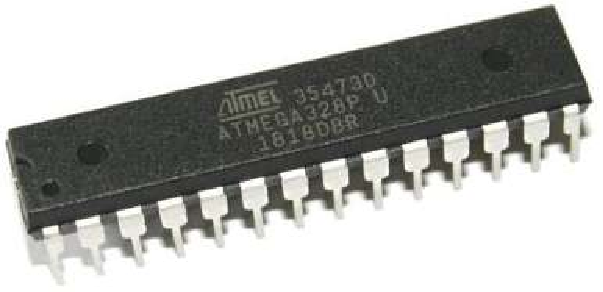
\includegraphics[scale=0.7]{micro.pdf}
	\caption{Microcontrolador Atmega328P utilizado.}
	\label{fig:img_micro}
\end{figure}


\subsection{Módulo de comunicación WiFi}

El módulo utilizado es el ESP-01, que es fabricado por Ai-Thinker y se basa en la familia de módulos WiFi “ESP8266” de Espressif Systems. El mismo se observa en la figura~\ref{fig:img_modWifi}. Este pequeño módulo puede utilizarse como adaptador Wi-Fi, que es la función que cumple en este proyecto. Mediante el mismo, se le agregó acceso inalámbrico a Internet al microcontrolador que maneja la placa, utilizando comunicación serie (USART). El módulo posee las siguientes características \cite{modwifi}:
\begin{itemize}
	\item Funciona en la banda de 2.4GHz
	\item Soporta WPA/ WPA2
	\item Rango de tensión de operación: 3 - 3.6V
	\item Consumo máximo de corriente: 170mA
	\item Puede funcionar como Estación, como Access Point (AP) o como ambas simultáneamente
\end{itemize}

Finalmente, el mismo posee ocho pines. Entre los mismos se encuentran un reset, un pin de habilitación, dos pines de alimentación y cuatro pines digitales, donde dos de ellos corresponden a una UART. En este proyecto, la UART se utiliza para la comunicación con el microcontrolador, mientras que uno de los pines digitales permite implementar una señal luminosa en caso de falla.
\begin{figure}[H]
	\centering
	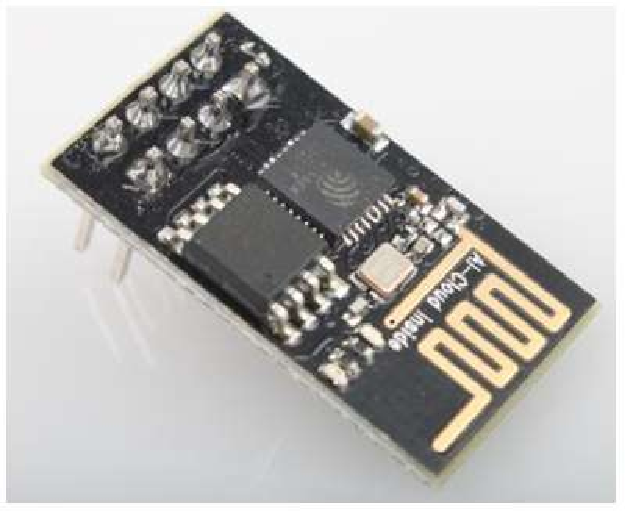
\includegraphics[scale=0.7]{modWifi.pdf}
	\caption{Módulo de comunicación  WiFi ESP-01 utilizado.}
	\label{fig:img_modWifi}
\end{figure}

\hl{ENCONTRAR Y VER SI SE ESCRIBE JUSTIFICACION SOBRE EL USO DE WIFI EN LUGAR DE OTRO PROTOCOLO. SI SE COMPLICA, SPEECH SOBRE POR QUE COSA PUEDE CAMBIARSE A FUTURO}


\section{Fuente de alimentación}
Este proyecto contempla el diseño y construcción de una fuente de tensión regulada. La misma se encarga de alimentar las barreras infrarrojas, el detector magnético, el microcontrolador y el módulo de comunicación WiFi. Para ello, cuenta con salidas de 12V, 5V y 3.3V de tensión continua. Fue implementada a partir de un transformador de 220Vac/12Vac. \textcolor{mGreen}{Su corriente de carga efectiva es X (medirla con el sistema completo conectado y funcionando).} El diagrama circuital de la fuente se observa en la figura ~\ref{fig:img_circuito_fuente}.
\begin{figure}[H]
	\centering
	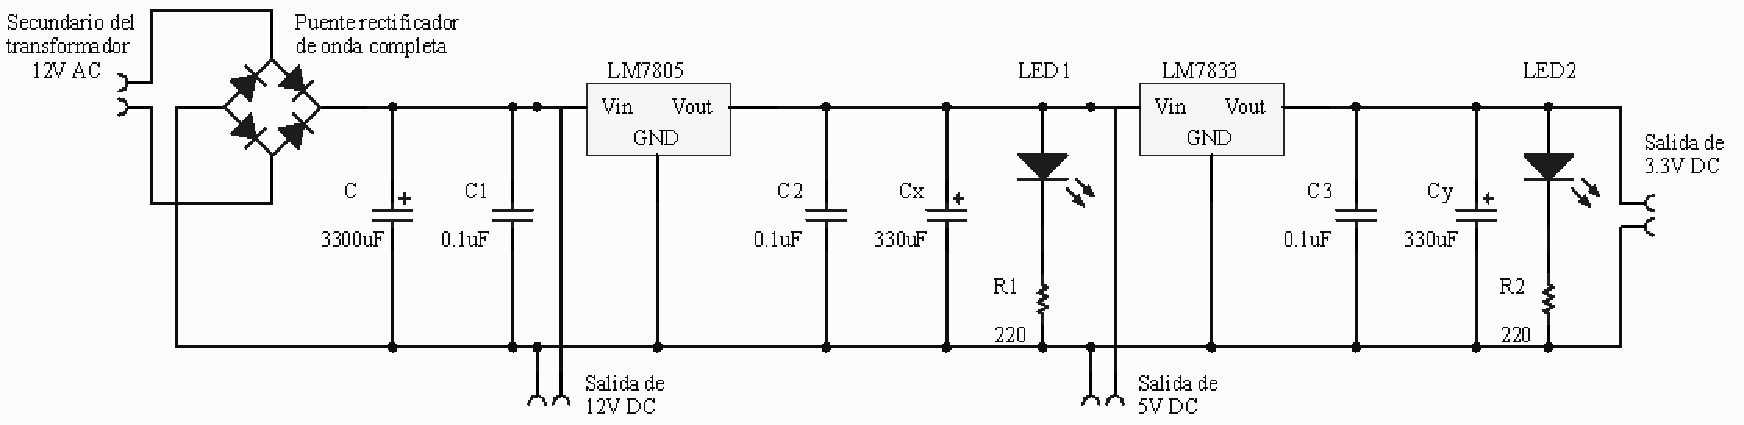
\includegraphics[width=\textwidth]{Circuito-fuente.pdf}
	\caption{Fuente de alimentación de tensión continua del sistema.}
	\label{fig:img_circuito_fuente}
\end{figure}

La fuente además cuenta con capacitores cerámicos y electrolíticos para filtrar los ruidos de alta y de baja frecuencia, respectivamente, que puedan ingresar al sistema a través de la misma, dado que se la utiliza para alimentar elementos externos, como es el caso de los periféricos (los cables actúan como antenas). 

Adicionalmente, se realizó el cálculo del disipador asociado al regulador de tensión LM7805 para que su temperatura no supere los $42^{\circ}$C. 

Finalmente, se cuenta con una protección frente a sobretensiones en el lado primario del transformador montada sobre la caja contenedora de la placa.


\section{Diseño de la etapa lógica y de comunicación}

El esquema circuital correspondiente a esta etapa se ilustra en la figura ~\ref{fig:img_circuito_logico}. Para garantizar el correcto funcionamiento del circuito básico integrado por el microcontrolador y el módulo de comunicación WiFi es necesario realizar ciertas conexiones en torno a cada uno de estos componentes.
%\textbf{OPCIÓN 2:} El esquema circuital correspondiente a esta etapa se ilustra en la figura ~\ref{fig:img_circuito_logico}. Para garantizar que el circuito básico integrado por el microcontrolador y el módulo de comunicación WiFi se encuentra en condiciones de ser encendido y comenzar a comunicarse es necesario realizar ciertas conexiones en torno a cada uno de estos componentes. 
Respecto al primero, se deben conectar las alimentaciones, un pulsador de reset y un oscilador de cristal. Este último está compuesto por un cristal de 16MHz y dos capacitores cerámicos de 22pF, como se indica en la tabla 6-3 de la hoja de datos del microcontrolador \cite{atmega328p}. El mismo es necesario para proveer al microcontrolador de una señal de reloj. En cuanto al módulo de comunicación WiFi, se debe realizar la conexión de la alimentación, el reset, el pin de habilitación y las líneas de transmisión y recepción.

\begin{figure}[H]
	\centering
	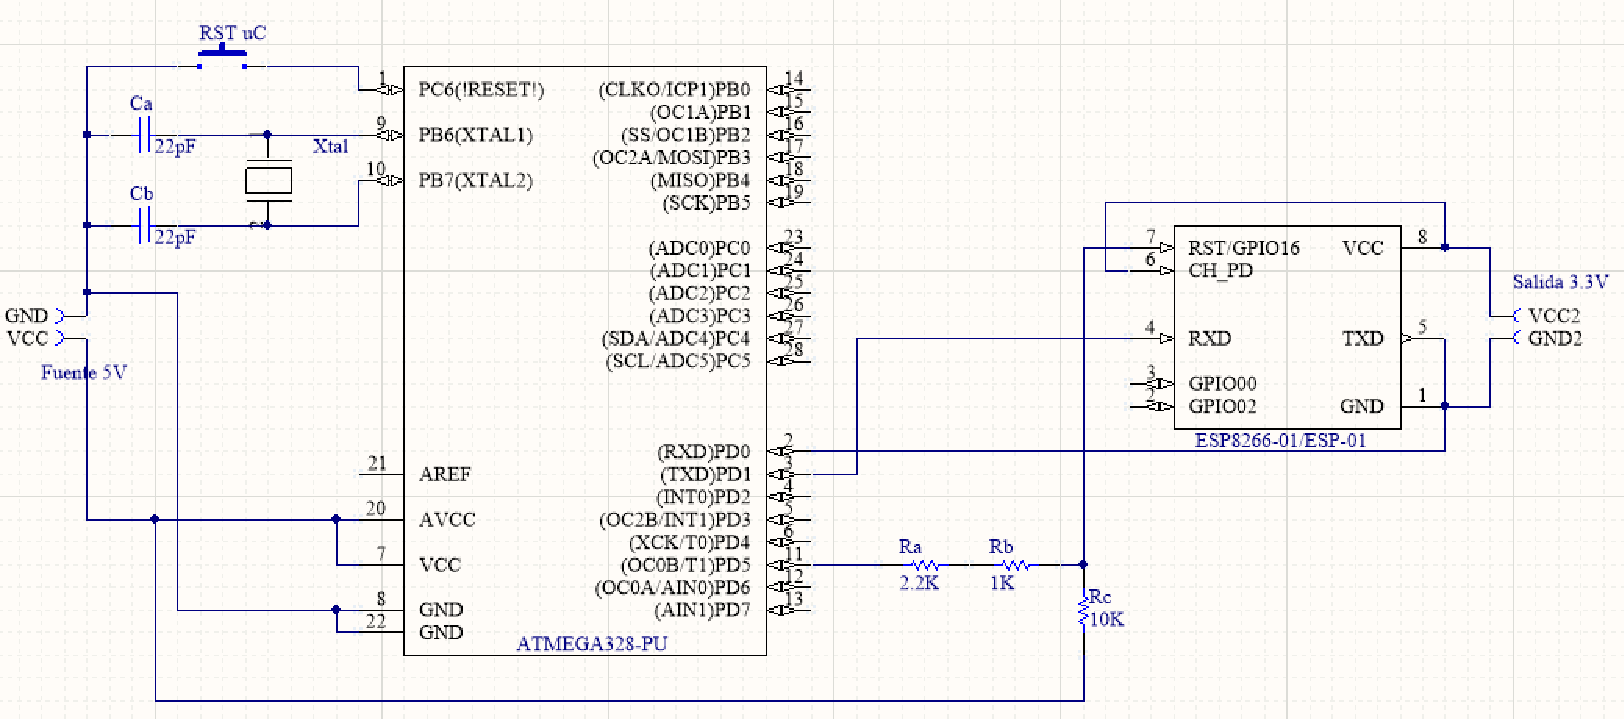
\includegraphics[width=\textwidth]{circuito-logico.pdf}
	\caption{Esquema circuital de la etapa de lógica y comunicación.}
	\label{fig:img_circuito_logico}
\end{figure}

En lo que respecta al conexionado de los periféricos que forman parte del sistema, se debe considerar el hecho de que algunos de ellos han sido simulados debido a una cuestión de costos o a que han quedado fuera del alcance del proyecto.

En cuanto a aquellos que se encuentran simulados, como es el caso de uno de los detectores magnéticos, las barreras vehiculares de entrada y salida y la expendedora de tickets del ingreso, la conexión con el microcontrolador es directa, mediante sus pines digitales de entrada. Mientras que la elevación de cada una de las barreras y la impresión del ticket se visualizan mediante un led, el segundo detector magnético y el retiro del ticket se simulan con pulsadores. 

Entre los que se encuentran verdaderamente implementados, que son las barreras infrarrojas que forman parte del sistema de detección de tamaño y uno de los sensores magnéticos de presencia, la conexión con el microcontrolador se realiza a través de una adaptación de niveles de tensión, como la de la figura~\ref{fig:img_Adapt_entradas_digitales}, para evitar dañar al mismo.

\begin{figure}[H]
	\centering
	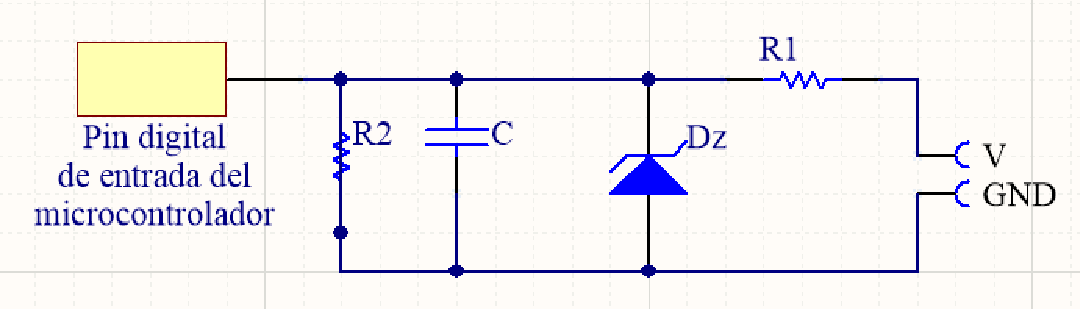
\includegraphics[width=\textwidth]{Adapt_entradas_digitales.pdf}
	\caption{Adaptación de niveles de tensión entre los periféricos y el microcontrolador.}
	\label{fig:img_Adapt_entradas_digitales}
\end{figure}

La función del diodo Zener es limitar la tensión máxima de entrada al pin digital a 5V, dado que en la hoja de datos se especifica que los mismos no admiten un valor superior a 5.5V. Esto se implementa debido a que los periféricos cuentan con contactos de relé que, en caso de cerrarse, envían al pin del microcontrolador los 12V con que son alimentados. Además, en caso de una inversión de la tensión de entrada, el Zener protege al microcontrolador ya que solo le entrega su tensión en directa, que son 0.6V aproximadamente.

Por otra parte, R1 se encarga de limitar la corriente que circulará por la adaptación, de manera de proteger al diodo Zener. El capacitor cerámico C, junto con R1 y R2, conforman un filtro que minimiza los ruidos provenientes desde el exterior del sistema, incluyendo los rebotes provocados por los relés de los periféricos. La resistencia R2 se coloca en paralelo a la impedancia de entrada del pin del microcontrolador por dos razones. Primero, para obtener una impedancia de entrada fija y aproximadamente del valor de R2. Segundo, para disminuir el ruido que ingresa al circuito integrado, dado que la tensión de ruido depende de la magnitud de la impedancia de entrada. Entonces, al reducir esta última colocándole una resistencia en paralelo, se disminuye el ruido de entrada.

Finalmente, la placa además cuenta con leds indicadores que se encienden en caso de producirse alguna falla en el microcontrolador o el módulo de comunicación WiFi.


\section{Diseño e implementación del PCB }

En esta sección se hace alusión a aquellas cuestiones relacionadas con el diseño y la implementación del circuito impreso. Para ello, fue utilizada la herramienta Altium Designer 19.0.15 con una licencia gratuita para estudiantes, la cual tiene validez por seis meses. 

Inicialmente, la Placa I/O fue implementada mediante una placa Arduino Mega. Esto se debió a que, en conjunto con docentes del Laboratorio de Comunicaciones (LAC), en el cual se desarrolló el proyecto, se determinó que la misma es una herramienta adecuada para llevar a cabo el diseño del prototipo del sistema. Las razones que motivaron esta elección son la disponibilidad de una gran cantidad de información acerca del tema, tanto en libros como en la web, en forma gratuita, y a que en el laboratorio se cuenta con personal que posee experiencia trabajando con este modelo de placa. Por otra parte, el microcontrolador ATmega2560 que la misma posee permite implementar el sistema planteado.

%Esto se debió a dos cuestiones. Primero, ante nuestra falta de conocimiento, tanto para la elección de microcontroladores como para su programación, docentes del Laboratorio de Comunicaciones (LAC), en el cual se está desarrollando el proyecto, consideraron que era una buena opción para empezar a incursionar en este tema. Esto se debe a que hay disponible una gran cantidad de información acerca del tema, tanto en libros como en la web, y en forma gratuita. Segundo, se determinó que el microcontrolador ATmega2560 que esta placa posee permite implementar el sistema planteado.

El uso de esta placa de desarrollo permitió ensayar el funcionamiento de los códigos que se fueron realizando al inicio del proyecto. Posteriormente, la misma fue reemplazada por un circuito construido utilizando protoboards. El mismo fue implementado con el microcontrolador ATmega328P. Esto se debió a que, a pesar de haber estado trabajando con el ATmega2560 que es superior, éste resulta adecuado para desempeñar las funciones requeridas por el prototipo que se obtendrá al final de este proyecto.  

Una vez que se verificó que el circuito desarrollado funcionaba en forma correcta, se procedió a realizar el diseño del PCB correspondiente. Durante el mismo, se creó la mayor parte de los encapsulados utilizados y, además, se recurrió a librerías disponibles en la página web oficial de Altium. Inicialmente se desarrolló un modelo esquemático, a partir del cual se obtuvo el circuito impreso del sistema. Con respecto a este último, fue necesario modificar algunas de las reglas de diseño establecidas por defecto, como es el caso del ancho de las pistas, la distancia entre ellas, y a distancia entre pistas y el plano de masa.

Con el objetivo de verificar si el ancho de las pistas elegido era adecuado, se recurrió a calculadoras de ancho de pista en función de la corriente y la sobreelevación de temperatura permitida. Debido a que la corriente de carga del sistema es baja, el ancho de pista de 0.7mm elegido resultó correcto.

Finalmente, la placa fue elaborada mediante el método de insolado. En un principio, se intentó fabricarla con la insoladora proporcionada por el LAC pero, luego de varios intentos fallidos debidos a la baja calidad de impresión del fotolito y del film fotosensible disponible, se decidió enviarla a un productor de PCB local. 

La placa construida se observa en la figura ~\ref{fig:img_pcb_imagen_tesis}.

\begin{figure}[H]
	\centering
	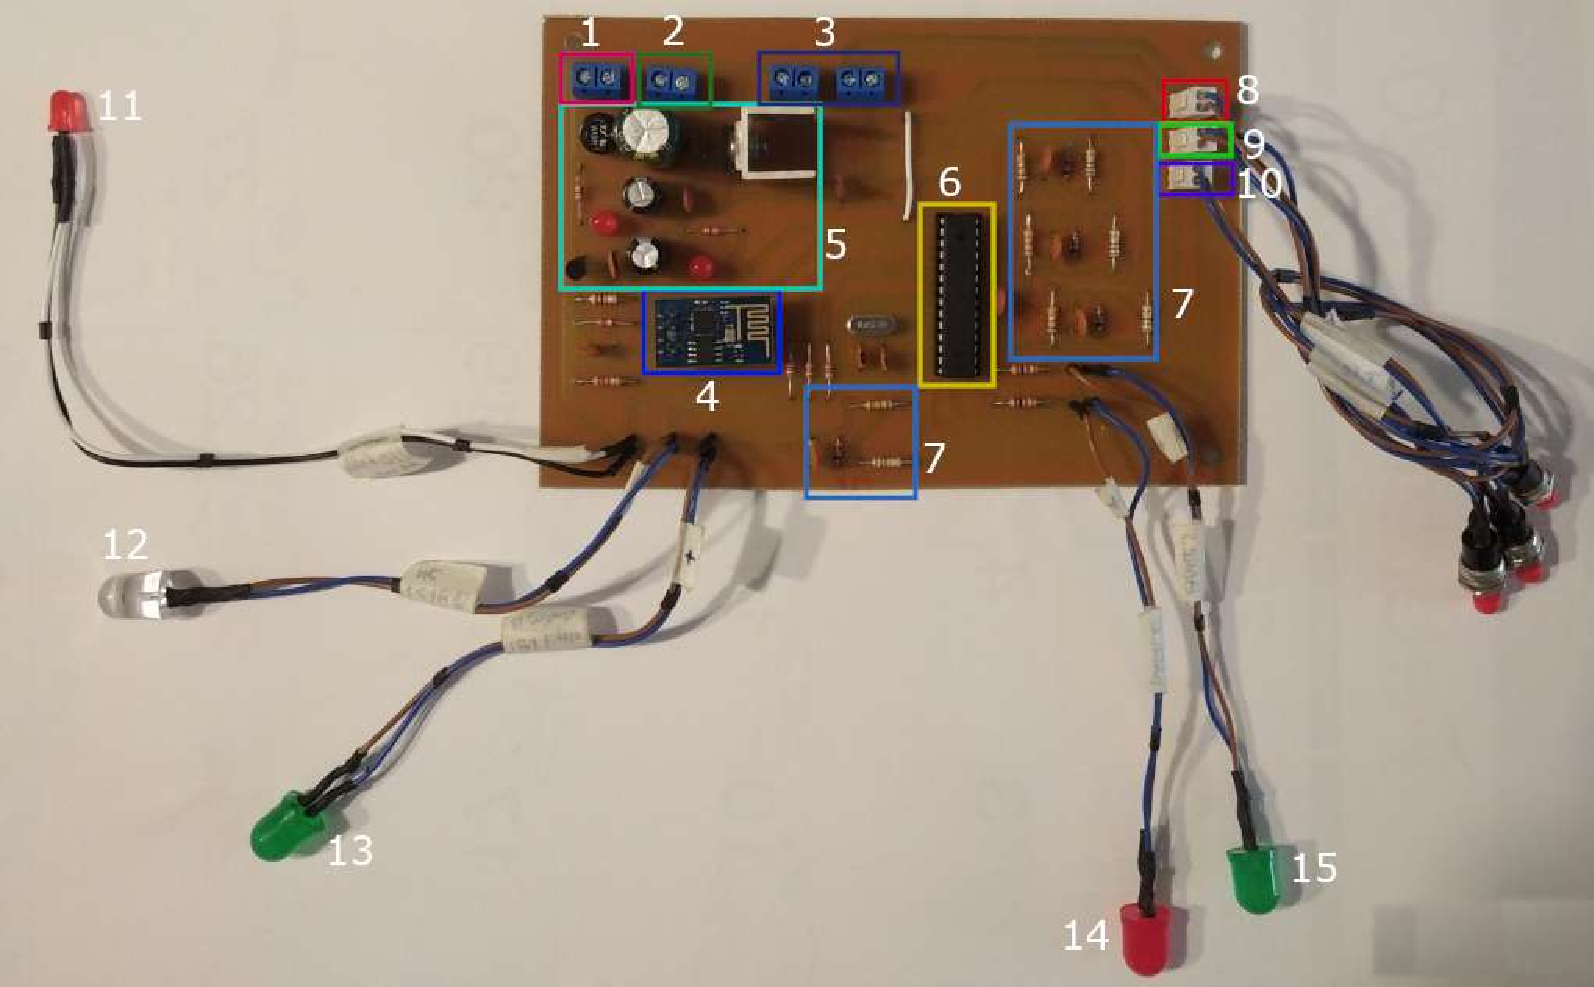
\includegraphics[width=\textwidth]{pcb_imagen_tesis.pdf}
	\caption{PCB generado a partir del diseño final.}
	\label{fig:img_pcb_imagen_tesis}
\end{figure}

Sobre la misma se ha indicado con recuadros de diversos colores las diferentes partes que la componen. Estas se detallan a continuación:

\begin{enumerate}
	\item Entrada de 12V de alterna, proveniente desde el bobinado secundario del transformador.
	\item Salida de 12V de continua destinada a la alimentación de los periféricos: las tres barreras infrarrojas y el detector magnético.
	\item Entradas provenientes desde los periféricos. Observando desde la izquierda se tiene: barrera infrarroja 3, barrera infrarroja 2, detector magnético y barrera infrarroja 1.
	\item Módulo de comunicación WiFi.
	\item Fuente regulada de tensión continua.
	\item Microcontrolador ATmega328P
	\item Adaptaciones de nivel de tensión entre los periféricos y los pines del microcontrolador.
	\item Pulsador de reset del microcontrolador.
	\item Pulsador para simulación del detector magnético de salida.
	\item Pulsador para simulación del retiro del ticket a la entrada.
	\item Led indicador de falla del Módulo WiFi.
	\item Led indicador de falla del Microcontrolador.
	\item Led para simulación de impresión del ticket.
	\item Led para simulación de barrera de entrada.
	\item Led para simulación de barrera de salida.
\end{enumerate}




\section{Periféricos}
En la presente sección, se realiza una breve descripción de los periféricos que forman parte del sistema, que fueron proporcionados por la empresa interesada en el desarrollo de este proyecto.

\subsection{Barreras Infrarrojas}

El sistema posee tres barreras infrarrojas que componen el sistema de detección de tamaño de los vehículos que desean ingresar a los establecimientos. Uno de esos equipos se observa en la figura~\ref{fig:img_Barrera_infrarroja}.

\begin{figure}[H]
	\centering
	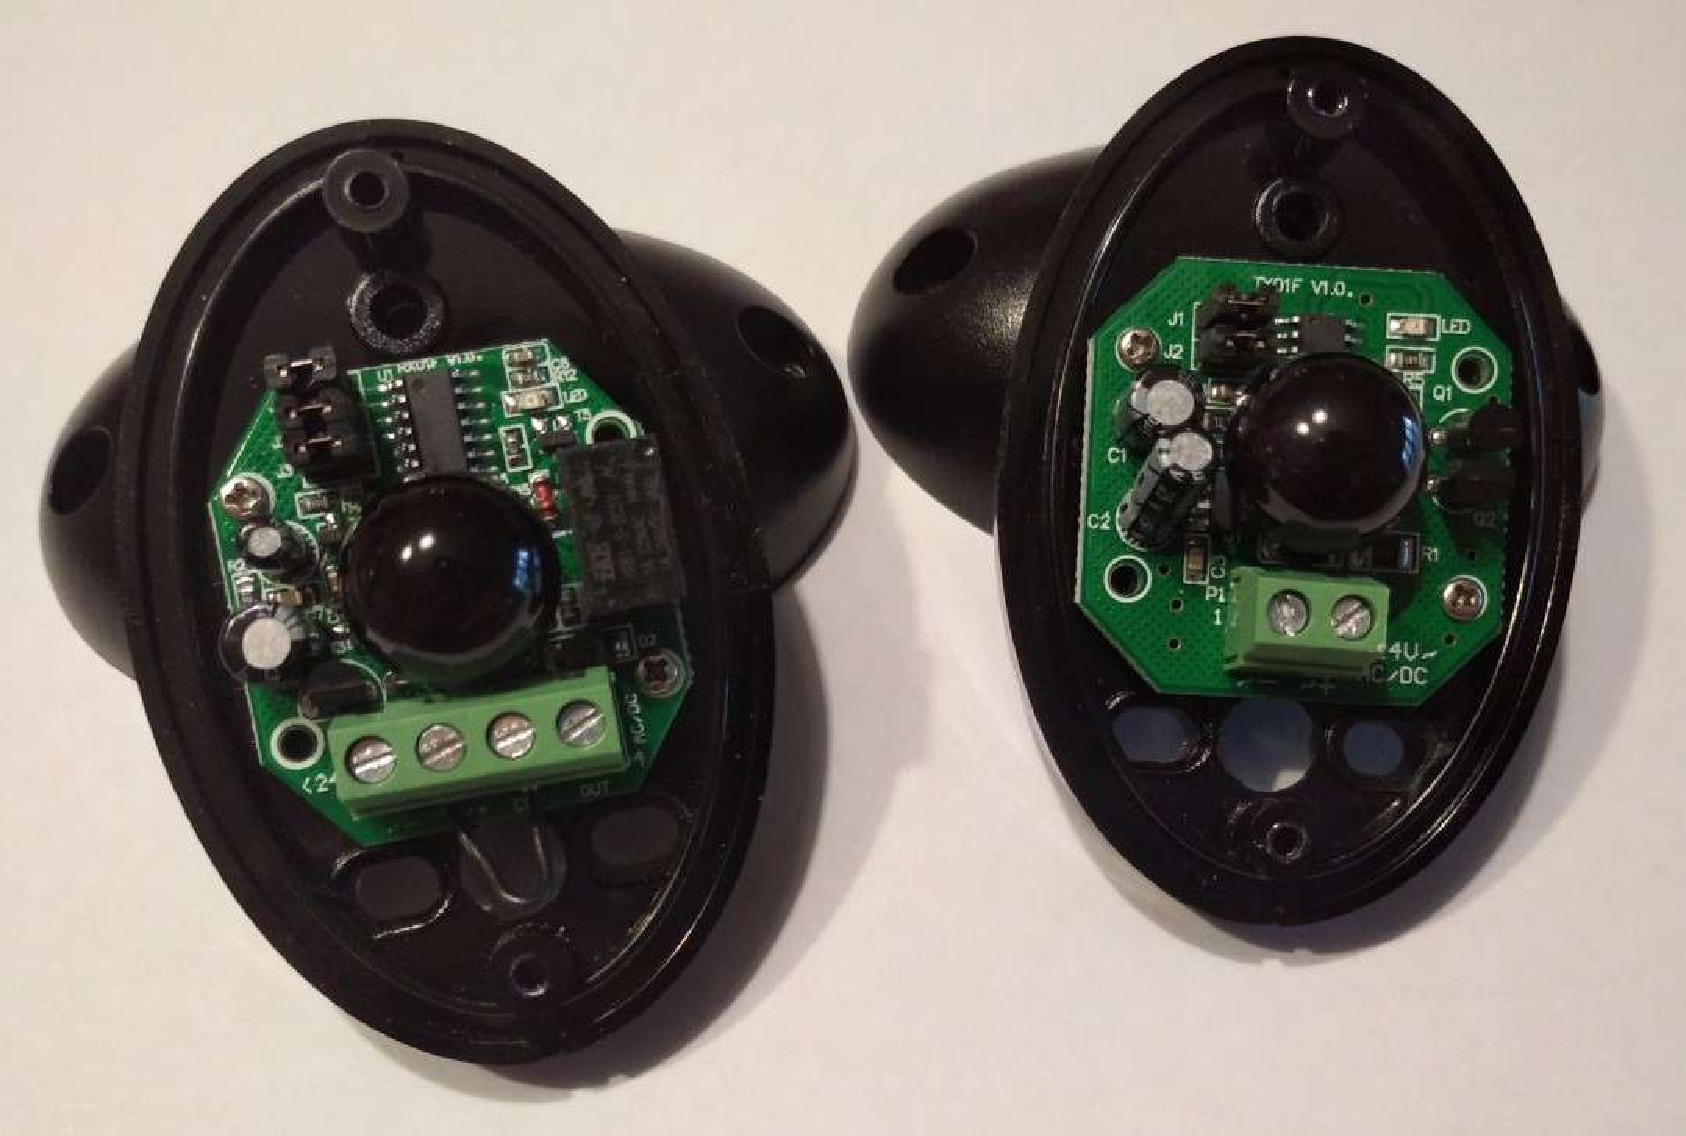
\includegraphics[scale=0.3]{Barrera_infrarroja.pdf}
	\caption{Barrera infrarroja utilizada: receptor (izquierda) y transmisor (derecha).}
	\label{fig:img_Barrera_infrarroja}
\end{figure}

Las características más relevantes de este modelo de barrera son las siguientes:
\begin{itemize}
	\item Alcance $\leq$ 15m
	\item Tensión de operación: DC/AC 12-24V
	\item Consumo de corriente del receptor: 15mA
	\item Consumo de corriente del transmisor: 30mA
\end{itemize}

Por otra parte, tanto el equipo transmisor como el receptor poseen dos jumpers J2 y J3. Estos se utilizan para determinar la frecuencia de trabajo de la barrera. A partir de los mismos, existen cuatro combinaciones correspondientes a cuatro frecuencias distintas. Esto permite que barreras cercanas trabajen a diferentes frecuencias y se evita que se produzcan interferencias entre ellas.

Adicionalmente, el receptor posee un jumper adicional J1 que se utiliza para determinar si el contacto disponible de su relé interno es el normal cerrado o el normal abierto.

En la figura~\ref{fig:img_Barrera_infrarroja}, se observa el diagrama de conexiones del receptor (izquierda) y del transmisor (derecha). Mientras el segundo únicamente requiere tensión de alimentación, el primero también posee el común y la salida del relé interno. En el sistema, el común se encuentra conectado a la tensión de alimentación para que, en caso de activarse la barrera, a la salida del relé se tengan los 12V de entrada. Estos 12V son acondicionados mediante la adaptación de niveles para que al microcontrolador lleguen 5V. 

\begin{figure}[H]
	\centering
	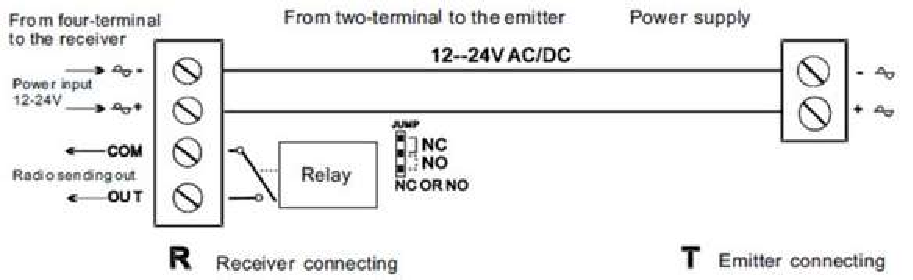
\includegraphics[width=\textwidth]{Conexion_barreras_infrarrojas.pdf}
	\caption{Conexiones de la barrera infrarroja: receptor (izquierda) y transmisor (derecha).}
	\label{fig:img_Conexion_barreras_infrarrojas}
\end{figure}

Finalmente, en lo que respecta al aseguramiento del correcto funcionamiento de este equipo, el mismo debe ser colocado al menos a 20cm de altura y con una distancia mayor a 1m entre receptor y transmisor.


\subsection{Detector de presencia magnético}

El sistema posee dos detectores de presencia magnéticos, aunque uno de ellos se encuentra simulado. Mientras que uno de ellos se ubica en el ingreso al establecimiento, el otro se encuentra en el egreso del mismo. Se lo puede observar en la figura~\ref{fig:img_Det_Mag}.

\begin{figure}[H]
	\centering
	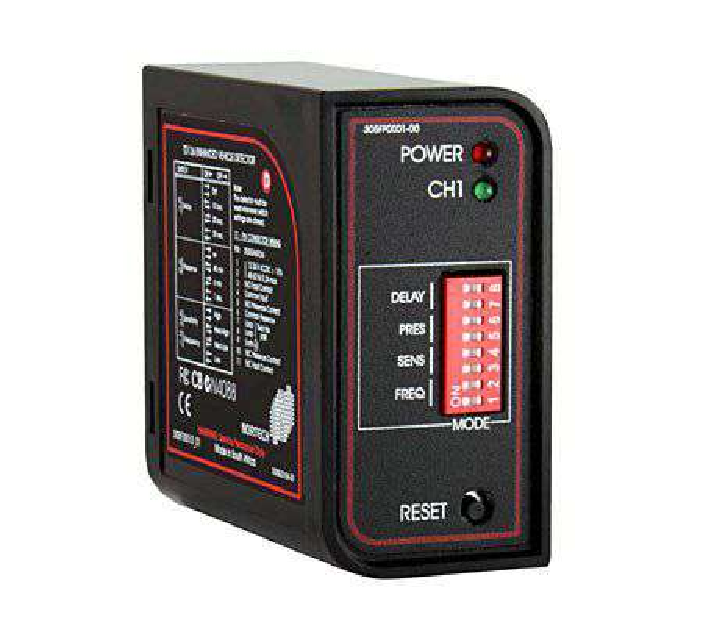
\includegraphics[scale=0.6]{Det_Mag.pdf}
	\caption{Detector magnético utilizado.}
	\label{fig:img_Det_Mag}
\end{figure}

Respecto al funcionamiento, al momento de darle alimentación, el detector se sintoniza automáticamente con el lazo inductivo que tiene conectado. El equipo requiere una tensión de alimentación de 12V DC/AC y \textcolor{mGreen}{tiene un consumo de corriente de X (verificarlo al probarlo)}.

Por otra parte, el equipo posee dos indicadores leds que se encenderán según el estado en el que el mismo se encuentra. Cuando está sintonizado, se encienden el led rojo (power) y el verde (detect). Luego de dos segundos, el verde se apaga. Por su parte, mientras el equipo se encuentre alimentado, el led rojo se encuentra siempre encendido. El verde, va a parpadear en caso de falla o va a quedar encendido cuando se detecte un vehículo atravesando el lazo.

El diagrama de conexiones se muestra en la figura ~\ref{fig:img_Conexiones_det_mag}. Los pines 1 y 2 están destinados a la alimentación del detector. Los pines 5, 6 y 10 forman parte del relé de presencia del sistema. Entre 5 y 6 se tiene el contacto normal abierto y entre 6 y 10 el normal cerrado. Los pines 3, 4 y 11 forman parte del relé de salida pulsada. Entre 3 y 4 se tiene el contacto normal abierto y entre 4 y 11 el normal cerrado. Al momento de detectar la presencia de un vehículo, puede utilizarse tanto la salida del relé de presencia como el de pulso. Mientras que el primero es energizado mientras el vehículo se encuentra sobre el lazo, el segundo lo hace cuando el vehículo ingresa al lazo o cuando sale de él. Esto último es configurable. Finalmente, entre los pines 7 y 8 se conecta el lazo inductivo.

\begin{figure}[H]
	\centering
	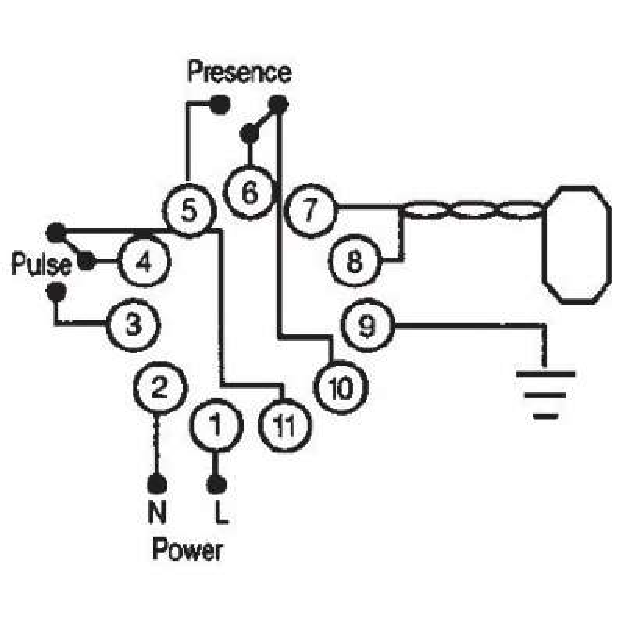
\includegraphics[scale=0.6]{Conexiones_det_mag.pdf}
	\caption{Conexiones de la barrera infrarroja: receptor (izquierda) y transmisor (derecha).}
	\label{fig:img_Conexiones_det_mag}
\end{figure}

Como se observa en la figura~\ref{fig:img_Det_Mag}, en el frente del detector hay 8 selectores que permiten configurar el equipo:
\begin{itemize}
	\item \textbf{Ajuste de frecuencia:} corresponde a los primeros dos selectores. Hay cuatro combinaciones o frecuencias posibles. Esto permite que detectores que están ubicados cerca operen a diferentes frecuencias y no interfieran entre sí.
	\item \textbf{Ajuste de sensibilidad:} corresponde a los siguientes tres selectores (3, 4 y 5). Hay ocho posibilidades, que hacen que el sensor sea más o menos selectivo al momento de realizar la detección.
	\item \textbf{Filtro:} permite eliminar las interferencias del entorno. Se lo activa seteando en ON el selector 6. Cuando se encuentra activado, el tiempo de reacción del detector aumenta y la sensibilidad se ve reducida. Es por esto que, a menos que el entorno lo requiera, no debe activarse.
	\item \textbf{Salida de relé:} corresponde al selector 7. Solo afecta a la salida del relé de pulso. Si se lo setea en OFF, el relé se energiza cuando un vehículo ingresa al lazo. En caso contrario, el mismo es energizado cuando el vehículo egresa del lazo. 
	\item \textbf{Tiempo de presencia:} corresponde al selector 8. Permite determinar si el relé de presencia mantiene la presencia detectada hasta que el vehículo deja el lazo o si lo hace solo por diez minutos.
\end{itemize}

En caso de hacer alguna modificación en la configuración es necesario volver a sintonizar el detector. Para ello, puede utilizarse el botón de reset.

Respecto al lazo inductivo, el mismo debe realizarse con cable de $1.5mm^{2}$ de área y debe tener forma rectangular. La cantidad de vueltas que posee depende de las dimensiones con las que se lo construya. Basándose en el manual de usuario y en el tamaño de las vías de acceso de los establecimientos relevados, en este proyecto se consideró el uso de un lazo de 2.5m de largo por 1m de ancho, al que le corresponden cuatro vueltas de cable. Adicionalmente, los extremos del cable del lazo debe trenzarse, con al menos veinte vueltas por metro. Esto último tiene por objetivo que el cable de conexión del lazo no forme parte del área de detección, evitando que participe de la misma.

En caso de que el detector no funcione correctamente, se debe proceder de la siguiente manera:
\begin{itemize}
	\item Verificar el estado del lazo inductivo y del cableado
	\item Modificar la sensibilidad y/o la frecuencia
	\item Setear el filtro en ON
\end{itemize}









